\documentclass[11pt,a4paper]{report}

% ---------------------------------------------------------------- layout
\usepackage[a4paper,margin=1in]{geometry}
\usepackage[T1]{fontenc}
\usepackage{lmodern}
\usepackage{amsmath,amssymb}
\usepackage{graphicx}
\usepackage{xcolor}
\usepackage{booktabs}
\usepackage{tabularx}
\usepackage{array}
\usepackage{enumitem}
\usepackage{caption}
\usepackage{subcaption}
\usepackage{listings}
\usepackage{needspace}
\usepackage[ruled,vlined,linesnumbered]{algorithm2e}
\usepackage[most]{tcolorbox}
\usepackage{tikz}
\usetikzlibrary{arrows.meta,positioning,fit,calc,shapes.geometric,backgrounds}
\usepackage{pgfplots}
\usepackage{pgfplotstable}
\usepgfplotslibrary{groupplots,statistics}
\pgfplotsset{compat=1.18}
\usepackage[colorlinks=true,linkcolor=blue!70!black,citecolor=green!45!black,urlcolor=blue!70!black]{hyperref}

\setlist{itemsep=2pt,topsep=4pt}

% ---------------------------------------------------------------- code listings
\definecolor{codebg}{HTML}{F2F1E9}
\definecolor{codekw}{HTML}{C7254E}
\definecolor{codestr}{HTML}{9C27B0}
\definecolor{codecom}{HTML}{3A8A3A}
\lstset{
  basicstyle=\ttfamily\small,
  backgroundcolor=\color{codebg},
  keywordstyle=\color{codekw},
  stringstyle=\color{codestr},
  commentstyle=\color{codecom}\itshape,
  numbers=left, numberstyle=\tiny\color{gray}, numbersep=6pt,
  xleftmargin=1.5em, framexleftmargin=1.5em, frame=none,
  columns=fullflexible, keepspaces=true, showstringspaces=false,
  breaklines=true, aboveskip=8pt, belowskip=8pt,
  escapeinside={(*@}{@*)}
}

% ---------------------------------------------------------------- boxes
\newtcolorbox{notebox}{enhanced, colback=gray!6, colframe=gray!70!black,
  boxrule=0.5pt, arc=2pt, title=Note, fonttitle=\small,
  left=6pt, right=6pt, top=4pt, bottom=4pt}
\newtcolorbox{defbox}[1]{enhanced, colback=blue!3, colframe=blue!45!black,
  boxrule=0.5pt, arc=2pt, title={#1}, fonttitle=\small\bfseries,
  left=6pt, right=6pt, top=4pt, bottom=4pt}

% ---------------------------------------------------------------- chart colours and styles
\definecolor{cstack}{HTML}{1BAF7A}
\definecolor{cstackdark}{HTML}{0F6E56}
\definecolor{cheap}{HTML}{2A78D6}
\definecolor{csize}{HTML}{EB6834}
\definecolor{cclass}{HTML}{6250D6}
\definecolor{celem}{HTML}{EDA100}
\definecolor{cunknown}{HTML}{9A9890}
\definecolor{inkc}{HTML}{52514E}
\definecolor{mutedc}{HTML}{898781}
\definecolor{gridc}{HTML}{E1E0D9}
\definecolor{basec}{HTML}{C3C2B7}

\newcommand{\NumBench}{7}
\newcommand{\LastBenchIdx}{6}
\newcommand{\AllIdx}{7}
\newcommand{\AllY}{7.4}
\newcommand{\TotalAllocs}{8{,}923}
\newcommand{\CandCount}{6{,}413}
\newcommand{\FailedCount}{2{,}510}
\newcommand{\StackCount}{31}
\newcommand{\CandRate}{71.9}
\newcommand{\StackRateOfCand}{0.48}
\newcommand{\HeapRateOfCand}{99.5}
\newcommand{\TopReason}{Size not const}
\newcommand{\TopReasonShare}{78.7}
\newcommand{\TopReasonShareAll}{22.1}
\newcommand{\StackXmax}{1.81}
\newcommand{\OkXmax}{2596}
\pgfplotsset{benchyticks/.style={ytick={0,1,2,3,4,5,6,7.4}}}
\pgfplotsset{benchonlyyticks/.style={ytick={0,1,2,3,4,5,6}}}
\expandafter\def\csname PanelTitle0\endcsname{eclipse\\failed = 526}
\expandafter\def\csname PanelTitle1\endcsname{fop\\failed = 235}
\expandafter\def\csname PanelTitle2\endcsname{h2\\failed = 471}
\expandafter\def\csname PanelTitle3\endcsname{jython\\failed = 229}
\expandafter\def\csname PanelTitle4\endcsname{lusearch\\failed = 279}
\expandafter\def\csname PanelTitle5\endcsname{sunflow\\failed = 374}
\expandafter\def\csname PanelTitle6\endcsname{xalan\\failed = 396}
\expandafter\def\csname PanelTitle7\endcsname{All\\failed = 2{,}510}

\pgfplotstableread[col sep=semicolon]{data/bench.csv}\benchtab

\pgfplotsset{
  base/.style={
    axis x line*=bottom, axis y line*=left,
    y axis line style={draw=none}, x axis line style={draw=basec},
    major tick style={draw=none},
    xmajorgrids, grid style={draw=gridc, line width=0.4pt},
    y dir=reverse,
    yticklabel style={font=\footnotesize, text=inkc},
    xticklabel style={font=\scriptsize, text=mutedc, /pgf/number format/1000 sep={}},
    xlabel style={font=\footnotesize, text=mutedc},
    title style={font=\small, align=left, anchor=south west, at={(0,1)}, yshift=1pt},
    legend style={draw=none, fill=none, font=\footnotesize, text=inkc, legend cell align=left,
                  /tikz/every even column/.append style={column sep=8pt}},
    legend image code/.code={\fill[##1] (0cm,-0.07cm) rectangle (0.22cm,0.13cm);},
    scaled x ticks=false,
  },
  benchrows/.style={base, clip=false, yticklabels from table={\benchtab}{name}, enlarge y limits={abs=0.6}},
  seg/.style={fill=#1, draw=white, line width=0.6pt},
  inseg/.style={
    point meta=explicit symbolic,
    nodes near coords={\pgfmathtruncatemacro\showlab{\pgfplotspointmeta>=10}%
      \ifnum\showlab=1 \pgfmathprintnumber[fixed,precision=0]{\pgfplotspointmeta}\%\fi},
    nodes near coords style={anchor=east, font=\scriptsize, text=white, inner sep=2pt},
  },
  endlab/.style={
    point meta=explicit symbolic,
    nodes near coords={\pgfplotspointmeta},
    nodes near coords style={anchor=west, font=\scriptsize, text=inkc, inner sep=2pt},
  },
}

% ---------------------------------------------------------------- tikz styles
\tikzset{
  blk/.style={draw, rounded corners=2pt, align=center, font=\small, inner sep=5pt},
  obj/.style={draw, minimum width=0.75cm, minimum height=0.5cm, font=\small, inner sep=1pt, fill=white},
  var/.style={draw, circle, minimum size=0.55cm, inner sep=0pt, font=\small},
  arr/.style={-{Stealth[length=5pt]}, thick},
}

\newcommand{\cv}[3]{\langle #1,\ #2,\ #3\rangle}

\renewcommand{\bibname}{References}
\begin{document}

% ================================================================ title page
\begin{titlepage}
  \centering
  \vspace*{1.5cm}
  {\LARGE\bfseries Memory Optimization in\\[4pt] Object-Oriented Programming Languages\par}
  \vspace{1.2cm}
  {\large CS-777 Report\par}
  \vspace{1.2cm}
  {\large Ashutosh Sharma\par}
  \vspace{4pt}
  {\large 26M2107\par}
  \vspace{1cm}
  {\normalsize Guide: Prof.\ Manas Thakur\par}
  \vfill
  {\large 23\textsuperscript{rd} November, 2026\par}
  \vspace{1cm}
  
\includegraphics[width=4.2cm]{figures/iitb-logo.png}\par
  \vspace{1cm}
  {\large Department of Computer Science and Engineering\par}
  {\large Indian Institute of Technology Bombay\par}
  \vspace*{0.5cm}
\end{titlepage}

\pagenumbering{arabic}
\tableofcontents
\clearpage

% ================================================================ abstract
\setcounter{page}{1}
\addcontentsline{toc}{section}{Abstract}
\begin{abstract}
    Java researchers have long struggled with a fundamental trade-off: whether to perform precise analyses within the JIT compiler or delegate them to the static compilation stage and leverage their results at runtime. \\
    \\
    Over the years, several efforts have been made to improve Escape Analysis (EA), enabling more objects to be allocated on the stack rather than the heap. However, much of this work has primarily focused on regular objects, leaving another significant category of Java objects, like arrays, relatively unexplored \\
    \\
    Arrays introduce an additional set of constraints that make them particularly challenging candidates for stack allocation. In this report, we examine these constraints, investigate the limitations they impose on existing Escape Analysis implementations, and outline potential directions for addressing some of these challenges as part of our future work.
\end{abstract}
\clearpage

\chapter{Introduction}

Managed object-oriented languages such as Java free the programmer from manual memory
management: objects are created with \texttt{new} and are reclaimed automatically once they
are no longer reachable. This convenience has a price. Every object lives on a garbage-collected
heap, every access to it goes through a reference, and the runtime must periodically stop or
slow down the program to collect garbage. A long line of work has therefore tried to move
short-lived objects off the heap and onto the call stack, where they are cheap to allocate,
cheap to access, and disappear as soon as the method that created them returns.

This report studies that optimization, \emph{stack allocation}, in the context of the Eclipse
OpenJ9 Java virtual machine~\cite{openj9}. In this chapter we first describe how Java programs
are executed and how memory is managed, then explain how escape analysis enables stack
allocation, and finally discuss why getting a precise escape analysis is hard both inside a JIT
compiler and in a static compiler.

\section{Java Execution Pipeline}

Java programs are executed in two stages (Figure~\ref{fig:pipeline}). In the \emph{static}
stage, the \texttt{javac} compiler translates source code into platform-independent
bytecode, stored in \texttt{.class} files. In the \emph{dynamic} stage, the Java virtual machine
(JVM) loads this bytecode on the target machine and executes it. Every method starts in the
interpreter; methods that are invoked often enough are handed to the just-in-time (JIT) compiler,
which translates them into optimized machine code. From then on, calls to that method run the
compiled code instead of the interpreter, which is where most of the program's performance
comes from.

\begin{figure}[htbp]
  \centering
  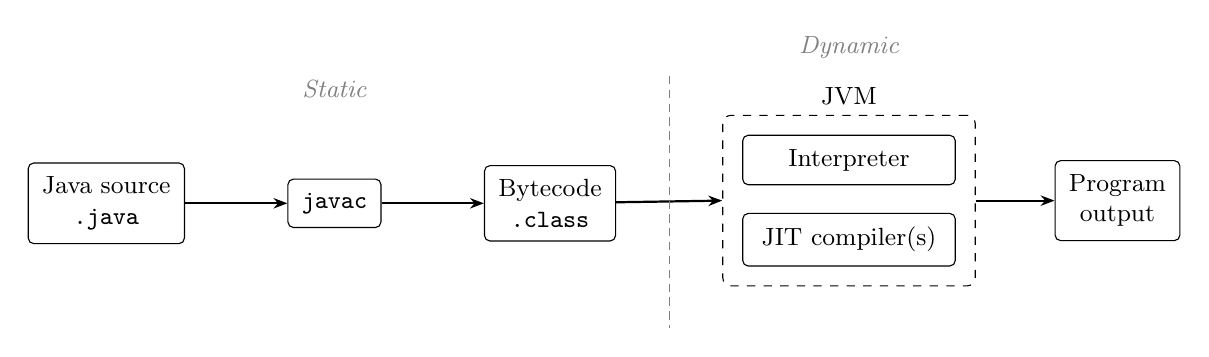
\begin{tikzpicture}[node distance=1.1cm]
    \node[blk] (src) {Java source\\\texttt{.java}};
    \node[blk, right=1.3cm of src] (javac) {\texttt{javac}};
    \node[blk, right=1.3cm of javac] (bc) {Bytecode\\\texttt{.class}};
    \node[blk, right=1.6cm of bc, yshift=0.55cm, minimum width=2.7cm] (interp) {Interpreter};
    \node[blk, below=0.35cm of interp, minimum width=2.7cm] (jit) {JIT compiler(s)};
    \node[draw, dashed, rounded corners=3pt, inner sep=7pt, fit=(interp)(jit),
          label={[font=\small]above:JVM}] (jvm) {};
    \node[blk, right=1.0cm of jvm] (out) {Program\\output};
    \draw[arr] (src) -- (javac);
    \draw[arr] (javac) -- (bc);
    \draw[arr] (bc) -- (jvm.west);
    \draw[arr] (jvm) -- (out);
    \draw[densely dashed, gray] ($(bc.east)!0.5!(jvm.west) + (0,1.6)$) -- ++(0,-3.2);
    \node[font=\small\itshape, gray] at ($(javac) + (0,1.45)$) {Static};
    \node[font=\small\itshape, gray] at ($(jvm.north) + (0,0.85)$) {Dynamic};
  \end{tikzpicture}
  \caption{Java execution pipeline. \texttt{javac} produces bytecode statically; the JVM's
           interpreter and JIT compiler execute it dynamically.}
  \label{fig:pipeline}
\end{figure}

This split is central to the rest of the report. Analyses can be performed either statically,
where time is plentiful but the final program (its libraries, its dynamically loaded classes) is
not fully known, or during JIT compilation, where the running program is known exactly but every
millisecond spent analysing it is added to the program's execution time.

\section{Java Memory Management}

By default, Java allocates every object on the heap. The heap is owned and managed by the
garbage collector, which dictates how memory is structured and handles both the allocation and
the deallocation of objects.

\paragraph{Benefits.} Automatic memory management eliminates manual allocation and
deallocation, and with it a whole class of memory bugs such as dangling pointers, double frees
and many memory leaks.

\paragraph{Costs.} Every heap object is reached through a reference, so accesses pay for an
extra indirection, and the garbage collector adds its own performance overhead: it must trace
live objects, reclaim dead ones, and in many designs pause the application while doing so.

\section{Stack Allocation via Escape Analysis}

The JIT compiler can reduce these costs with \emph{escape analysis}.
Escape analysis determines the set of objects that do not \emph{escape} their allocating method,
that is, objects that are never stored into a location reachable after the method returns (a
static field, a heap object, the return value, or an argument of an unknown callee). Such
objects can be allocated on the method's stack frame instead of the heap. Stack-allocated
objects:
\begin{itemize}
  \item have a lower access time, since they live in the frame of the method using them; and
  \item are freed as soon as the allocating method returns, without any work from the garbage
        collector.
\end{itemize}

\paragraph{Limitations in OpenJ9.} OpenJ9's JIT compiler performs escape analysis and stack
allocation, but with two important limitations:
\begin{itemize}
  \item it is triggered only at the hotter optimization levels, so methods that are compiled
        only at lower levels never benefit from it; and
  \item it is intraprocedural, with a limited ability to ``peek'' into callees. Any call it
        cannot see through must be treated conservatively, which makes the analysis imprecise.
\end{itemize}

\section{Precision Challenges in Both Realms}
\label{sec:challenges}

A natural idea is to compute escape information more precisely. Doing so is hard in both stages
of the pipeline.

\paragraph{Challenges with JIT analysis.} The time spent in JIT compilation is added to the
execution time of the program. JIT compilers therefore trade precision for efficiency: they use
fast, local analyses rather than expensive whole-program ones.

\paragraph{Challenges with static analysis.} A static analysis can afford to be expensive, but it
faces two problems of its own:
\begin{itemize}
  \item a precise whole-program analysis needs the code of library methods, which may not be
        available (or may differ) when the application is compiled; and
  \item an object that the static analysis marks as stack-allocatable might still escape at run
        time, because of dynamic language features such as \emph{dynamic class loading},
        \emph{hot-code replacement}, and \emph{callbacks} into application code.
\end{itemize}

The work surveyed in Chapter~\ref{ch:literature} addresses both sets of challenges by splitting
the analysis between the static compiler and the JIT compiler.

\section{Organization of this Report}

Chapter~\ref{ch:literature} surveys two staged static\,+\,JIT approaches: the PYE framework and
optimistic stack allocation with dynamic heapification. Chapter~\ref{ch:toolbox} describes the
tools we use: the Soot analysis framework and OpenJ9's debug counters.
Chapter~\ref{ch:experiments} presents two experiments on OpenJ9, one on how well the stack-frame
budget for stack-allocated objects is used and one on why arrays are rarely stack allocated.
Chapter~\ref{ch:conclusion} concludes and outlines future research directions.

\chapter{Literature Survey}
\label{ch:literature}

Both works surveyed in this chapter follow the same high-level idea: perform the expensive,
precise analysis \emph{statically}, ship its results with the program, and let the JIT compiler
use them cheaply at run time. They differ in what they do about the two problems raised in
Section~\ref{sec:challenges}: PYE handles missing library code, while optimistic stack allocation
handles dynamic features that can invalidate static results.

\section{The PYE Framework}

PYE (\emph{Precise-Yet-Efficient}) by Thakur and Nandivada~\cite{thakur2019pye} is a two-stage
(static\,+\,JIT) analysis framework for Java programs. Its key contributions are:
\begin{itemize}
  \item a way to record dependences between the application and the libraries it calls,
        called \emph{conditional values};
  \item offloading the expensive part of the analysis to the static compiler, which produces
        \emph{partial summaries} expressed in terms of conditional values; and
  \item enabling highly precise analysis results that the JIT compiler can evaluate cheaply at
        run time, once the actual libraries are known.
\end{itemize}

\subsection{Architecture}

Figure~\ref{fig:pye} shows the two halves of PYE.

\begin{figure}[htbp]
  \centering
  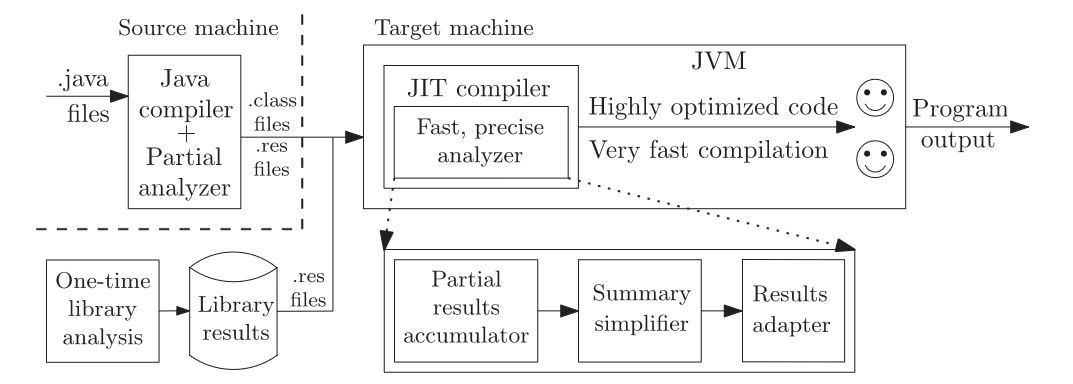
\includegraphics[width=0.9\linewidth]{figures/pye_architecture.png}
  \caption{Architecture of PYE (adapted from~\cite{thakur2019pye}). The static side writes
           partial summaries to \texttt{.res} files; the JIT side combines them with library
           summaries to obtain final results.}
  \label{fig:pye}
\end{figure}

\paragraph{Static compiler + partial analyzer.} On the source machine, PYE performs a precise
analysis of the application. Calls to library methods, whose code may not be available or may
change before the program runs, are \emph{skipped} rather than approximated. The resulting
partial summaries are written to \texttt{.res} files that ship with the \texttt{.class} files.
Library methods are analysed once, separately, in the same way.

\paragraph{JIT compiler + fast-precise analyzer.} On the target machine, when the JIT compiler
compiles a method, it reads only the summaries it needs, resolves the dependences between
application and library summaries, and populates the relevant JVM data structures with the final
results. Since all of the heavy lifting has already happened statically, this step is fast.

\subsection{Conditional Values}

A traditional summary maps each object in a method to a single data-flow value; for escape
analysis this is \textsc{Escape} or \textsc{NoEscape}. When part of the program is missing, such
a summary must be conservative. PYE's partial summaries instead map each element of a method's
domain to a \emph{set of conditional values}.

\begin{defbox}{Definition 1 (Conditional value)}
A conditional value is a triple
\[ T = \langle \Theta,\ \mathit{val},\ \mathit{val}' \rangle, \]
where
\begin{itemize}
  \item $\Theta = \langle u, x \rangle$, with $u$ a method and $x$ a program element in $u$; and
  \item $\mathit{val}, \mathit{val}' \in \mathit{Val}$, the set of values of the data-flow equations.
\end{itemize}
It reads: \emph{if element $x$ of method $u$ has value $\mathit{val}$, then the element being
summarized has value $\mathit{val}'$}.
\end{defbox}

Consider the method in Listing~\ref{lst:cv}, where \texttt{bar} is a library method that is not
available during static analysis.

\begin{minipage}[t]{0.47\textwidth}
\begin{lstlisting}[language=Java, caption={Example for conditional values.}, label={lst:cv}]
void foo(A p) {
  A a = new A();   // O1
  A b = new A();   // O2
  A c = new A();   // O3
  bar(b);          // library method
  c.g = 10;
}
\end{lstlisting}
\end{minipage}\hfill
\begin{minipage}[t]{0.48\textwidth}
\vspace{10pt}
\centering
\begin{tabular}{@{}ll@{}}
  \toprule
  Object & Conditional values \\
  \midrule
  $O_1$ & $\emptyset$ \quad (never escapes) \\
  $O_2$ & $\{\cv{\langle \mathit{bar}, p_0\rangle}{E}{E}\}$ \\
  $O_3$ & $\emptyset$ \quad (never escapes) \\
  \bottomrule
\end{tabular}
\end{minipage}

\medskip
Objects $O_1$ and $O_3$ never leave \texttt{foo}, so they need no condition. Object $O_2$ is
passed to \texttt{bar}; whether it escapes depends entirely on what \texttt{bar} does with its
first parameter $p_0$. Instead of giving up and marking $O_2$ as escaping, PYE records the
conditional value $\cv{\langle \mathit{bar}, p_0\rangle}{E}{E}$: \emph{$O_2$ escapes if and
only if $p_0$ escapes in \texttt{bar}}. At run time the JIT compiler looks up the summary of the
actual \texttt{bar}, evaluates the condition, and obtains a precise answer.

\section{Optimistic Stack Allocation and Dynamic Heapification}

Anand et al.~\cite{anand2024optimistic} build on the same static\,+\,JIT idea to improve stack
allocation in OpenJ9. Their approach has three key ideas:
\begin{itemize}
  \item it performs stack allocation \emph{optimistically}, using the results of a precise
        static escape analysis;
  \item it handles the cases that violate the optimistic assumptions at run time through
        \emph{dynamic heapification}; and
  \item it uses static analysis to optimize the \emph{ordering} of objects on the stack, reducing
        the run-time overhead of heapification checks.
\end{itemize}

\subsection{Optimistic Stack Allocation}

\paragraph{Static escape analysis (offline).} The static analysis is context-, flow- and
field-sensitive. It builds points-to graphs and a call graph, and computes method summaries
bottom-up over the call graph.

\paragraph{Passing results to the runtime.} The JIT compiler and the static analysis must agree
on how objects are named. Objects are identified by the \emph{bytecode index} (BCI) of their
allocation site, which is the same in the static compiler and in the JVM. For every method, the
BCIs of non-escaping allocation sites are stored in a \texttt{.res} file.

\paragraph{OpenJ9 JIT integration.} The \texttt{.res} file is loaded once, at JVM start-up. When
the JIT compiler runs its own escape analysis on a method, it may conclude that an object escapes
(for example, because it is passed to a callee the JIT cannot see through) even though the static
analysis says it does not. Such objects become \emph{additional} candidates and are
optimistically added to the stack-allocation candidate list.

\subsection{Motivating Example}

Optimism is only safe as long as the program behaves the way the static analysis assumed.
Listing~\ref{lst:heapify} shows a case where it does not.

\needspace{22\baselineskip}
\begin{lstlisting}[language=Java, caption={Dynamic class loading invalidates a static escape result.}, label={lst:heapify}]
class A {
  A f;
  void foo(A q, A r) {
    A x = new A();   // O4
    A y = new A();   // O5
    x.f = new A();   // O6
    A p = x.f;
    bar(p, y);
    r.zar(p, q);
  }
  void zar(A p, A q) { ... }   // does not leak p
  void bar(A p1, A p2) {
    p1.f = p2;
  }
}
class B extends A {            // dynamically loaded
  void zar(A p, A q) {
    q.f = p;                   // leaks p into q
  }
}
\end{lstlisting}

When the program is analysed statically, only \texttt{A.zar} is known, and it does not leak its
arguments. Inside \texttt{foo}, $O_4$ is reachable only from the local \texttt{x}, $O_6$ only
through \texttt{x.f} (and the local \texttt{p}), and $O_5$ only through \texttt{y} and, after
\texttt{bar}, through \texttt{O6.f}. None of them escapes, so \textbf{$O_4$, $O_5$ and $O_6$ are
allocated on the stack optimistically} (Figure~\ref{fig:pts}, left).

Now suppose class \texttt{B} is loaded at run time and \texttt{r} refers to a \texttt{B}. The
call \texttt{r.zar(p, q)} then executes \texttt{q.f = p}, storing $O_6$ into an object owned by
the caller (Figure~\ref{fig:pts}, right). $O_6$ now escapes \texttt{foo}, and so does $O_5$,
which is reachable from $O_6$ through its field \texttt{f}. Leaving them on the stack would leave
the caller holding a dangling reference once \texttt{foo} returns.

\begin{figure}[htbp]
  \centering
  \begin{subfigure}[b]{0.4\textwidth}
    \centering
    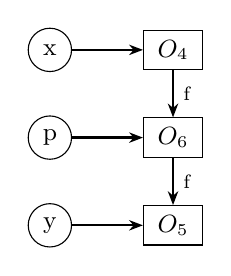
\begin{tikzpicture}[node distance=0.55cm and 0.9cm]
      \node[var] (x) {x};
      \node[obj, right=of x] (o4) {$O_4$};
      \node[var, below=of x] (p) {p};
      \node[obj, right=of p] (o6) {$O_6$};
      \node[var, below=of p] (y) {y};
      \node[obj, right=of y] (o5) {$O_5$};
      \draw[arr] (x) -- (o4);
      \draw[arr] (p) -- (o6);
      \draw[arr] (y) -- (o5);
      \draw[arr] (o4) -- node[right, font=\scriptsize] {f} (o6);
      \draw[arr] (o6) -- node[right, font=\scriptsize] {f} (o5);
    \end{tikzpicture}
    \caption{Static view: nothing escapes.}
  \end{subfigure}
  \qquad
  \begin{subfigure}[b]{0.4\textwidth}
    \centering
    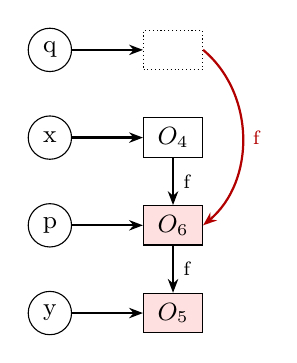
\begin{tikzpicture}[node distance=0.55cm and 0.9cm]
      \node[var] (q) {q};
      \node[obj, right=of q, densely dotted] (qo) {};
      \node[var, below=of q] (x) {x};
      \node[obj, right=of x] (o4) {$O_4$};
      \node[var, below=of x] (p) {p};
      \node[obj, right=of p, fill=red!12] (o6) {$O_6$};
      \node[var, below=of p] (y) {y};
      \node[obj, right=of y, fill=red!12] (o5) {$O_5$};
      \draw[arr] (q) -- (qo);
      \draw[arr] (x) -- (o4);
      \draw[arr] (p) -- (o6);
      \draw[arr] (y) -- (o5);
      \draw[arr] (o4) -- node[right, font=\scriptsize] {f} (o6);
      \draw[arr] (o6) -- node[right, font=\scriptsize] {f} (o5);
      \draw[arr, red!70!black] (qo.east) to[bend left=50] node[right, font=\scriptsize] {f} (o6.east);
    \end{tikzpicture}
    \caption{After \texttt{B.zar} runs: $O_6$ and $O_5$ escape.}
  \end{subfigure}
  \caption{Points-to graph of \texttt{foo} from Listing~\ref{lst:heapify}. The dotted box is the
           caller's object referenced by \texttt{q}.}
  \label{fig:pts}
\end{figure}

\subsection{Dynamic Heapification}

To stay correct, the runtime must detect such situations and move the affected objects off the
stack before the frame disappears. This is \emph{dynamic heapification}. Checks are placed at
reference stores: when a stack-allocated object is about to be written into a location outside
the current frame (for example, a field of a heap object or of an object in a caller's frame),
the object is copied to the heap. Because objects reachable from it may escape as well, the
process is applied transitively, and every reference that still points to the old stack copy is
updated to point to the new heap copy.

Figure~\ref{fig:heapify} shows the result for our example. $O_6$ and $O_5$ are heapified; the
field \texttt{f} of $O_4$ (which legitimately stays on the stack), the field \texttt{f} of the
new heap copy of $O_6$, and the local \texttt{y} are all redirected to the heap copies.

\begin{figure}[htbp]
  \centering
  
\includegraphics[width=0.9\linewidth]{figures/pldi_6.png}
  \caption{Architecture of PYE (adapted from~\cite{thakur2019pye}). The static side writes
           partial summaries to \texttt{.res} files; the JIT side combines them with library
           summaries to obtain final results.}
  \label{fig:pye}
\end{figure}

These checks are executed on every reference store in optimistically compiled code, so their
cost matters. The third idea of the paper addresses this: the static analysis is also used to
choose the \emph{order} in which objects are laid out on the stack, which reduces the run-time
overhead of the heapification checks.

\subsection{Evaluation}

The authors evaluate their implementation in OpenJ9 on the DaCapo 23.11-Chopin~\cite{blackburn2025rethinking}
and DaCapo 9.12-MR1~\cite{blackburn2006dacapo} benchmark suites and on SPECjvm2008~\cite{specjvm2008}.
Table~\ref{tab:anand-eval} summarizes the improvements they report.

\begin{table}[htbp]
  \centering
  \begin{tabular}{@{}llll@{}}
    \toprule
    Metric & Measured as & Unit & Reported change \\
    \midrule
    Stack allocation & objects allocated on the stack & count & $+71\%$ \\
    Garbage collection & time spent in GC & s & $-5.3\%$ \\
    Performance & execution time & s & $-8.8\%$ \\
    \bottomrule
  \end{tabular}
  \caption{Results reported by Anand et al.~\cite{anand2024optimistic}. More stack allocation means
           fewer heap allocations, which lowers GC time and overall execution time.}
  \label{tab:anand-eval}
\end{table}

\section{Discussion}

These results suggest that stack allocation is worth pursuing further:
\begin{itemize}
  \item it delivers significant performance improvements on real benchmarks;
  \item it is backed by active research that is mature enough to build on but leaves room for
        new contributions, and the baselines and tooling (an OpenJ9 implementation, a static
        analysis, benchmark set-ups) already exist; and
  \item it unlocks further optimization opportunities.
\end{itemize}
Two directions stand out as natural next steps, and they are the subject of our experiments in
Chapter~\ref{ch:experiments}: making smarter use of the fixed stack-frame budget available for
stack-allocated objects, and extending the analysis (static and dynamic) to \emph{arrays}.

\chapter{Our Toolbox}
\label{ch:toolbox}

This chapter describes the two tools we rely on: the Soot framework for static analysis of Java
bytecode, and OpenJ9's debug counters for measuring what the JIT compiler does.

\section{Soot}

Soot~\cite{vallee2010soot} is a framework for analysing and transforming Java bytecode. It lifts
bytecode into \emph{Jimple}, a typed three-address intermediate representation, performs
analyses and optimizations on Jimple, and writes the optimized program back as bytecode. The
static escape analysis used by optimistic stack allocation~\cite{anand2024optimistic} and the
static half of PYE~\cite{thakur2019pye} are both implemented in Soot.

\paragraph{Data-flow analysis framework.} Soot provides a generic data-flow analysis framework:
\begin{itemize}
  \item it is template driven: the analysis writer supplies the flow set, the flow functions, the
        merge function and the direction (forward or backward);
  \item Soot then computes the fixed point itself, using worklists; and
  \item it provides further utilities such as def-use chains, points-to analysis and call-graph
        construction.
\end{itemize}

\subsection{Why a Three-Address Code?}

Java bytecode is a stack-based instruction set: most instructions take their operands from an
implicit operand stack and push their results back onto it. This hides the data flow.
Table~\ref{tab:tac} shows the bytecode of a small method that creates a \texttt{Point} and
returns the sum of its coordinates, the state of the operand stack after each instruction, and
the corresponding three-address code (TAC).

In bytecode the operands are implicit, so to find out what \texttt{iadd} adds, or which
\texttt{new} reaches the local \texttt{p}, an analysis must simulate the operand stack. In TAC
every statement performs one operation on explicit operands, so the data flow can be read
directly. This is why Soot's analyses, including escape analysis, work on Jimple rather than on
bytecode.

\section{OpenJ9 Debug Counters}

To understand what the JIT compiler does on real programs, we use OpenJ9's \emph{debug counters},
a utility for counting arbitrary events inside the JIT compiler. There are two kinds:
\begin{itemize}
  \item \textbf{Static} counters are incremented at compile time; nothing is added to the
        generated code. They count compile-time events, such as how many allocation sites were
        rejected for a given reason.
  \item \textbf{Dynamic} counters insert counter increments into the generated code, so they
        count how often an event happens at run time.
\end{itemize}

Counter names are hierarchical: a `\texttt{/}' in a name works like a slash in a file path and
expresses containment. When the counters are printed, each parent counter shows the total of its
children, and each child also shows its percentage of that parent. Listing~\ref{lst:dbg} and
Table~\ref{tab:dbg} show an example.

\begin{lstlisting}[language=C++, caption={Counting inlined and non-inlined call sites.}, label={lst:dbg}]
prependDebugCounter("callSites/inlined", tt);
...
prependDebugCounter("callSites/notInlined", tt);
\end{lstlisting}

\begin{table}[htbp]
  \centering
  \begin{tabular}{@{}rlrr@{}}
    \toprule
    & Counter & Count & \% \\
    \midrule
    1: & \texttt{callSites}             & 10000 & -- \\
    2: & \texttt{callSites/inlined}     & 8000  & 80.00\% \\
    3: & \texttt{callSites/notInlined}  & 2000  & 20.00\% \\
    \bottomrule
  \end{tabular}
  \caption{Output produced by the counters in Listing~\ref{lst:dbg}.}
  \label{tab:dbg}
\end{table}

Both experiments in Chapter~\ref{ch:experiments} use static debug counters.

\chapter{Experiments}
\label{ch:experiments}

This chapter presents two experiments on the OpenJ9 JIT compiler. The first asks whether the
fixed stack-frame budget for stack-allocated objects is a real constraint in practice. The
second asks why so few arrays are stack allocated.

\section{Investigating Stack-Frame Utilization}

OpenJ9 limits the stack-frame space available for stack-allocated objects to a fixed threshold
of \textbf{3000 bytes per method}. When the total size of all eligible candidates exceeds this
limit, escape analysis must remove some of them from the candidate list, and those objects are
allocated on the heap instead. The current implementation decides which candidates to remove
using object size alone, starting with the largest objects (Algorithm~\ref{alg:evict}).

\begin{algorithm}[htbp]
  \caption{Candidate eviction in OpenJ9 (size-based)}
  \label{alg:evict}
  \SetKwProg{Proc}{Procedure}{}{}
  \Proc{\textsc{EvictCandidates}(candidates, MAX)}{
    $\mathit{total} \leftarrow$ size of all candidates on the stack\;
    \While{$\mathit{total} > \mathit{MAX}$}{
      $c \leftarrow$ largest contiguous candidate \tcp*{size only}
      \If{no such $c$}{
        $c \leftarrow$ largest non-contiguous candidate\;
      }
      $\mathit{total} \leftarrow \mathit{total} - \mathit{size}(c)$\;
      mark $c$ as heap-allocated\;
    }
  }
\end{algorithm}

This raises two questions:
\begin{itemize}
  \item Is object size alone a good criterion for choosing which objects to remove?
  \item Does the current heuristic lead to suboptimal stack-frame utilization or suboptimal
        performance on real-world workloads?
\end{itemize}

\subsection{Candidate Eviction: An Example}

Listing~\ref{lst:evict} shows a method with three stack-allocation candidates. $O_1$ is used in
a hot loop, while $O_2$ and $O_3$ are allocated only in a block that runs when \texttt{n} is
zero.

\needspace{15\baselineskip}
\begin{lstlisting}[language=Java, caption={A method whose candidates exceed the budget.}, label={lst:evict}]
double work(int n) {
  Vec acc = new Vec();          // O1, 1600 B
  for (int i = 0; i < n; i++) {
    acc.add(i);                 // hot
  }
  if (n == 0) {                 // cold block
    Cfg a = new Cfg();          // O2, 1000 B
    Log b = new Log();          // O3,  800 B
    a.use(b);
  }
  return acc.sum();
}
\end{lstlisting}

Together the candidates need 3400\,B against a budget of 3000\,B, so at least 400\,B must be
evicted. Table~\ref{tab:evict} compares the current rule with a hot-path-aware rule that evicts
the coldest candidate first, and the smallest among candidates that are equally cold.

\begin{table}[htbp]
  \centering
  \begin{tabular}{@{}llll@{}}
    \toprule
    Rule & Evicts & Stays on stack & Stack space used \\
    \midrule
    Largest-first (current) & $O_1$ & $O_2$, $O_3$ & 1800\,B \\
    Hot-path aware          & $O_3$ & $O_1$, $O_2$ & 2600\,B \\
    \bottomrule
  \end{tabular}
  \caption{Effect of two eviction rules on the method in Listing~\ref{lst:evict}.}
  \label{tab:evict}
\end{table}

The size-based rule evicts $O_1$, the one object that is used on the hot path, and keeps two
objects that are almost never allocated. A rule that takes execution frequency into account keeps
the hot object on the stack and also uses more of the budget. Whether this matters in practice
depends on how often real methods actually exceed the budget, which is what our first experiment
measures.

\section{Experiment 1: Stack-Frame Utilization}

\paragraph{Objective.} Find out whether real-world programs ever need more stack space for
stack-allocated objects than the budget allows.

\paragraph{What we measure.} For every compiled method:
\begin{itemize}
  \item how often the stack-allocation candidates exceed the budget ($\mathit{totalSize} >
        \mathit{MAX}$); and
  \item by how much they exceed it, or how much of the budget is left unused (the
        \emph{deficit}, $\mathit{totalSize} - \mathit{MAX}$).
\end{itemize}

\paragraph{How.} Two static debug counters per method, updated once, when that method is
compiled. From the deficit we compute each method's \emph{utilization}: the share of the
3000\,B budget actually taken by its stack-allocated objects.

\paragraph{Workload.} The DaCapo 9.12-MR1-bach benchmark suite~\cite{blackburn2006dacapo}:
large, varied Java applications whose access patterns are close to those of real-world software.

\subsection{Results}

Figure~\ref{fig:util} summarizes the utilization of every compiled method, per benchmark.

\begin{figure}[htbp]
\centering
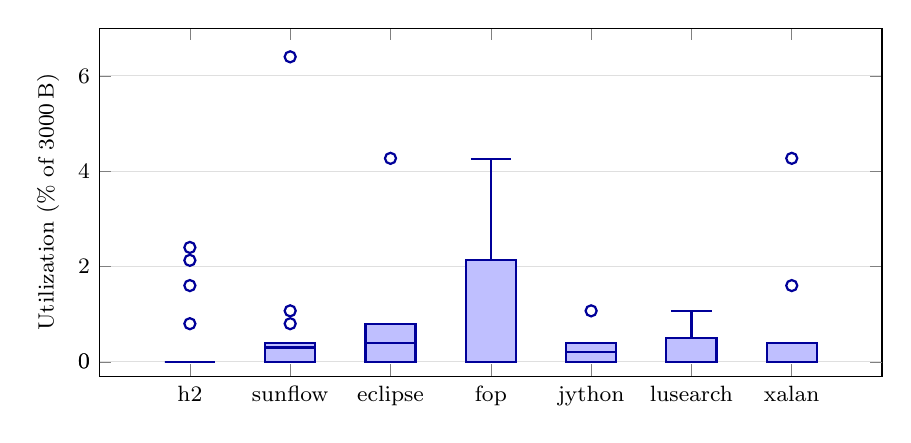
\begin{tikzpicture}
\begin{axis}[
    width=0.95\textwidth, height=6cm,
    boxplot/draw direction=y,
    ymin=-0.3, ymax=7,
    xtick={1,2,3,4,5,6,7},
    xticklabels={h2, sunflow, eclipse, fop, jython, lusearch, xalan},
    x tick label style={font=\footnotesize}, y tick label style={font=\footnotesize},
    ylabel={\footnotesize Utilization (\% of 3000\,B)},
    ymajorgrids, grid style={gray!25},
    boxplot={box extend=0.5},
    every boxplot/.style={fill=blue!25, draw=blue!60!black, solid, line width=0.8pt},
    extra y ticks={0}, extra y tick style={grid=none},
]
\addplot+[boxplot prepared={lower whisker=0.0, lower quartile=0.0, median=0.0,
          upper quartile=0.0, upper whisker=0.0}, mark=o, solid]
          coordinates {(1,0.8) (1,1.6) (1,2.13) (1,2.4)};
\addplot+[boxplot prepared={lower whisker=0.0, lower quartile=0.0, median=0.3,
          upper quartile=0.4, upper whisker=0.4}, mark=o, solid]
          coordinates {(2,0.8) (2,1.07) (2,6.4)};
\addplot+[boxplot prepared={lower whisker=0.0, lower quartile=0.0, median=0.4,
          upper quartile=0.8, upper whisker=0.8}, mark=o, solid]
          coordinates {(3,4.27)};
\addplot+[boxplot prepared={lower whisker=0.0, lower quartile=0.0, median=0.0,
          upper quartile=2.13, upper whisker=4.26}, mark=o, solid]
          coordinates {};
\addplot+[boxplot prepared={lower whisker=0.0, lower quartile=0.0, median=0.2,
          upper quartile=0.4, upper whisker=0.4}, mark=o, solid]
          coordinates {(5,1.07)};
\addplot+[boxplot prepared={lower whisker=0.0, lower quartile=0.0, median=0.0,
          upper quartile=0.5, upper whisker=1.06}, mark=o, solid]
          coordinates {};
\addplot+[boxplot prepared={lower whisker=0.0, lower quartile=0.0, median=0.0,
          upper quartile=0.4, upper whisker=0.4}, mark=o, solid]
          coordinates {(7,1.6) (7,4.27)};
\end{axis}
\end{tikzpicture}
\caption{Stack-frame utilization per compiled method. Each point is one method: the share of its
         3000\,B budget used by stack-allocated objects. Box: middle 50\% of methods; line:
         median; whiskers: typical range; circles: outlier methods.}
\label{fig:util}
\end{figure}

The budget is far from being a constraint. The median method uses at most 0.4\% of it (12\,B)
in every benchmark, and in h2, fop, lusearch and xalan at least half of the methods use none of
it at all; in h2 the whole box sits at zero, so at least three quarters of its methods use no
stack space. The largest value observed across all benchmarks is 6.4\% (192\,B), in sunflow. In
other words, no compiled method came close to the 3000\,B limit, and the eviction heuristic of
Algorithm~\ref{alg:evict} did not need to run for any method we observed.

\begin{notebox}
The question raised by the eviction example is therefore moot for this suite: a better eviction
rule cannot help when nothing is evicted. The more pressing problem is the opposite one: stack
frames stay \emph{under-utilized}, because few objects are admitted as candidates in the first
place.
\end{notebox}

\section{Array Stack-Allocation Opportunities}

Stack frames stay under-utilized in most methods, yet arrays are admitted to the candidate list
only under strict conditions, and arrays that fail these checks go to the heap even when they
never escape. This leads to two questions:
\begin{itemize}
  \item Why are arrays most often rejected from the candidate list?
  \item Can we be more aggressive with arrays?
\end{itemize}

\subsection{Eligibility of Arrays}

An array allocation is rejected as a stack-allocation candidate for one of two families of
reasons.

\paragraph{Element class unresolved or unknown.}
\begin{itemize}
  \item \emph{Not known at compile time}: the element class is only decided at run time, for
        example when the array is created reflectively.
  \item \emph{Not resolved}: the element class is known but has not been resolved yet, for
        example because the allocation sits on a path the interpreter never executed before the
        method was compiled.
\end{itemize}
Primitive arrays always pass these checks: their element types are known and loaded at VM
start-up.

\paragraph{Array size.}
\begin{itemize}
  \item \emph{Zero length}.
  \item \emph{Not a constant}: the length is only decided at run time.
  \item \emph{Too large}: the length is above a threshold.
\end{itemize}
These checks exist because a stack frame needs a size fixed at compile time, and a single array
must not use up the whole budget. The question, then, is which of these constraints rejects the
most arrays in real programs.

\section{Experiment 2: Why Arrays Are Rejected}

\paragraph{Objective.} Find the reasons arrays do not make it into the candidate list.

\paragraph{What we measure.}
\begin{itemize}
  \item the percentage of candidate arrays that are actually stack allocated; and
  \item the number of array allocations rejected, for each rejection reason.
\end{itemize}

\paragraph{How.} We added an enumeration listing every possible rejection reason, and one static
debug counter per reason, incremented at the point where the array is rejected. Counters are
organised hierarchically under \texttt{ArrayAlloc}; Listing~\ref{lst:h2counters} shows the raw
output for h2. The reasons map to the labels used in the rest of this section as follows:
\texttt{ArraySizeNotConst} is \emph{dynamic size}, \texttt{ClassUnresolved} is \emph{class
unresolved}, \texttt{ElementClassNotLoadaddr} is \emph{element class not known}, and every other
rejection is counted as \emph{unknown}.

\begin{lstlisting}[language={}, numbers=none, basicstyle=\ttfamily\scriptsize, caption={Static debug counters for h2.}, label={lst:h2counters}]
ArrayAlloc                                              |  1195
ArrayAlloc/ArrayCandidateFailed                         |   471 |  39.41%
ArrayAlloc/ArrayCandidateFailed/ArraySizeNotConst       |   413 |  34.56% |  87.69%
ArrayAlloc/ArrayCandidateFailed/ClassUnresolved         |    31 |   2.59% |   6.58%
ArrayAlloc/ArrayCandidateFailed/ElementClassNotLoadaddr |     2 |   0.17% |   0.42%
ArrayAlloc/ArrayCandidateFailed/Unknown                 |    25 |   2.09% |   5.31%
ArrayAlloc/ArrayCandidateOk                             |   718 |  60.08%
ArrayAlloc/StackAllocated                               |     6 |   0.50%
\end{lstlisting}

\paragraph{Workload.} The DaCapo 9.12-MR1-bach benchmark suite, with 20 iterations per
benchmark. Only compiled methods are counted, so the runs must be long enough for the JIT
compiler to warm up.

\subsection{Results}

Table~\ref{tab:arrays} lists the raw counts. Throughout, the number of array allocations
analysed in a benchmark is the sum of the rejected arrays and the candidate arrays, and the
stack-allocated arrays are counted as a subset of the candidates.\footnote{In every benchmark
the top-level \texttt{ArrayAlloc} counter equals \emph{rejected + candidates + stack allocated}
exactly (for h2, $471 + 718 + 6 = 1195$), which suggests that \texttt{StackAllocated} may be
counted separately from \texttt{ArrayCandidateOk}. If so, the stack-allocation rates below
would change only in the second decimal place (for h2, $6/724$ instead of $6/718$).}

\begin{table}[htbp]
  \centering
  \small
  \setlength{\tabcolsep}{5pt}
  \begin{tabular}{@{}lrrrrrrrr@{}}
    \toprule
    & & \multicolumn{2}{c}{Candidates} & \multicolumn{5}{c}{Rejected} \\
    \cmidrule(lr){3-4} \cmidrule(l){5-9}
    Benchmark & Analysed & Total & Stack & Total & Dyn.\ size & Class unres. & Elem.\ class & Unknown \\
    \midrule
    eclipse  & 2{,}689 & 2{,}163 & 6 & 526 & 392 & 85 & 3 & 46 \\
    fop      & 965     & 730     & 4 & 235 & 180 & 39 & 2 & 14 \\
    h2       & 1{,}189 & 718     & 6 & 471 & 413 & 31 & 2 & 25 \\
    jython   & 920     & 691     & 2 & 229 & 164 & 45 & 2 & 18 \\
    lusearch & 762     & 483     & 0 & 279 & 240 & 27 & 2 & 10 \\
    sunflow  & 1{,}269 & 895     & 9 & 374 & 304 & 49 & 3 & 18 \\
    xalan    & 1{,}129 & 733     & 4 & 396 & 282 & 71 & 2 & 41 \\
    \midrule
    All      & 8{,}923 & 6{,}413 & 31 & 2{,}510 & 1{,}975 & 347 & 16 & 172 \\
    \bottomrule
  \end{tabular}
  \caption{Array allocations in compiled methods of the DaCapo 9.12-MR1 benchmarks.}
  \label{tab:arrays}
\end{table}

\paragraph{Candidates are rarely stack allocated.} Most array allocations, \CandRate\% overall,
do pass the candidacy checks. Yet very few of these candidates end up on the stack
(Figure~\ref{fig:stackarrays}): across all benchmarks only \StackCount{} of \CandCount{}
candidate arrays (\StackRateOfCand\%) are stack allocated, and lusearch stack-allocates none.
Passing the candidacy checks is therefore far from sufficient; the arrays are lost at a later
stage of escape analysis.

\begin{figure}[htbp]
  \centering
  \begin{tikzpicture}
    \begin{groupplot}[
        group style={group size=2 by 1, horizontal sep=2.0cm, yticklabels at=edge left},
        benchrows, benchyticks, height=6.2cm, /pgf/bar width=8pt, xmin=0]

      \nextgroupplot[xbar stacked, width=7.4cm, xmax=\OkXmax,
                     title={Candidate arrays (count)},
                     legend columns=2, legend style={at={(1.15,1.18)}, anchor=south}]
      \addplot[seg=cheap] table[x=okheap, y=ypos]{\benchtab};
      \addplot[seg=cstack, endlab] table[x=okstack, y=ypos, meta=oklab]{\benchtab};
      \legend{Not stack allocated (heap), Stack allocated}

      \nextgroupplot[xbar, /pgf/bar shift=0pt, width=6.6cm, xmax=\StackXmax,
                     title={\% of candidates stack allocated}]
      \addplot[fill=cstack, draw=none, endlab,
               restrict expr to domain={\coordindex}{0:\LastBenchIdx}]
        table[x=stackpct, y=ypos, meta=stacklab]{\benchtab};
      \addplot[fill=cstackdark, draw=none, endlab,
               restrict expr to domain={\coordindex}{\AllIdx:\AllIdx}]
        table[x=stackpct, y=ypos, meta=stacklab]{\benchtab};
    \end{groupplot}
  \end{tikzpicture}
  \caption{Stack allocation of candidate arrays. Left: candidate arrays per benchmark, split into
           heap and stack allocated (the stack-allocated part is too small to be visible). Right:
           the share of candidates that is stack allocated.}
  \label{fig:stackarrays}
\end{figure}

\paragraph{Dynamic size dominates the rejections.} Figure~\ref{fig:reasons} breaks the rejected
arrays down by reason. A size that is not a compile-time constant is by far the most common
reason, accounting for \TopReasonShare\% of all rejections (1{,}975 of \FailedCount{}), and for
between 71\% and 88\% in every individual benchmark. An unresolved element class is a distant
second at 13.8\% overall (6.6\% to 19.7\% per benchmark). Arrays whose element class is not
known at compile time are rare (16 in total), consistent with reflective array creation being
uncommon in hot code.

\begin{figure}[htbp]
  \centering
  \begin{tikzpicture}
    \begin{axis}[benchrows, benchyticks, xbar stacked, /pgf/bar width=8pt,
                 width=0.86\textwidth, height=6.4cm, xmin=0, xmax=100,
                 xlabel={\% of rejected array allocations},
                 legend columns=4, legend style={at={(0.5,1.03)}, anchor=south}]
      \addplot[seg=csize,    inseg] table[x=p_size,    y=ypos, meta=p_size]{\benchtab};
      \addplot[seg=cclass,   inseg] table[x=p_class,   y=ypos, meta=p_class]{\benchtab};
      \addplot[seg=celem,    inseg] table[x=p_elem,    y=ypos, meta=p_elem]{\benchtab};
      \addplot[seg=cunknown, inseg] table[x=p_unknown, y=ypos, meta=p_unknown]{\benchtab};
      \addplot[draw=none, fill=none, forget plot, endlab]
        table[x expr=0.001, y=ypos, meta=failedlab]{\benchtab};
      \legend{Dynamic size, Class unresolved, Element class not known, Unknown}
    \end{axis}
  \end{tikzpicture}
  \caption{Reasons why array allocations are rejected as stack-allocation candidates; $n$ is the
           number of rejected arrays in each benchmark.}
  \label{fig:reasons}
\end{figure}

\subsection{Discussion}

The two experiments point in the same direction. The per-method budget is almost never the
limiting factor; what limits stack allocation of arrays is, first, that 28\% of all array allocations
are rejected as candidates, mostly because their size is not a compile-time
constant, and second, that almost none of the arrays that \emph{are} candidates end up on the
stack. Both gaps are targets for the research directions in the next chapter.

\chapter{Conclusion and Future Work}
\label{ch:conclusion}

In this report we studied stack allocation of objects in Java, an optimization that reduces both
the access cost of objects and the load on the garbage collector. We surveyed two staged
static\,+\,JIT approaches that make the JIT compiler's escape analysis more precise without
making it slower: PYE, whose conditional values let a static analysis summarize methods despite
missing library code, and optimistic stack allocation with dynamic heapification, which acts on
static escape results at run time and repairs the cases where dynamic features such as class
loading invalidate them. The latter reports a 71\% increase in stack allocations, a 5.3\%
reduction in GC time and an 8.8\% reduction in execution time.

We then used OpenJ9's debug counters to look at how stack allocation behaves on the DaCapo
benchmarks. The 3000\,B per-method budget for stack-allocated objects is far from exhausted: no
compiled method used more than 6.4\% of it, so the size-based eviction heuristic never came into
play. Arrays, on the other hand, rarely reach the stack. Only \StackRateOfCand\% of candidate
arrays are stack allocated, and \TopReasonShare\% of the arrays rejected as candidates are
rejected because their size is not a compile-time constant.

\section{Future Work}

These observations suggest the following research directions.

\paragraph{Arrays of dynamic size (\TopReasonShare\% of rejections).}
\begin{itemize}
  \item Use profiling information to find arrays whose size turns out to be constant, or bounded,
        at run time, and reserve stack-frame space for them. A method is typically recompiled
        several times as it gets hotter, so profile data collected during earlier executions is
        available to later, more optimized compilations.
  \item Add heapification checks wherever such an array may be reallocated, so that the program
        stays correct when a run-time size does not fit the reserved space.
  \item Statically identify arrays that are never reallocated, and skip the heapification checks
        for them.
\end{itemize}

\paragraph{Large arrays.} Split large arrays into chunks in the style of arraylets (a spine that
points to fixed-size leaves), so that the chunks fit into the stack-frame budget. The trade-off is
one extra indirection on every element access.

\paragraph{The candidate-to-stack gap.} Most candidate arrays still end up on the heap. Finding
out where in escape analysis they are lost, and why, may well be the larger opportunity, and it
is a prerequisite for knowing how much the two directions above can gain.


% ================================================================ references
\begin{thebibliography}{9}
\addcontentsline{toc}{chapter}{References}

\bibitem{anand2024optimistic}
Aditya Anand, Solai Adithya, Swapnil Rustagi, Priyam Seth, Vijay Sundaresan, Daryl Maier,
V.~Krishna Nandivada, and Manas Thakur.
Optimistic stack allocation and dynamic heapification for managed runtimes.
\emph{Proc.\ ACM Program.\ Lang.}, 8(PLDI), June 2024.
\url{https://doi.org/10.1145/3656389}.

\bibitem{blackburn2006dacapo}
Stephen~M. Blackburn, Robin Garner, Chris Hoffmann, Asjad~M. Khang, Kathryn~S. McKinley,
Rotem Bentzur, Amer Diwan, Daniel Feinberg, Daniel Frampton, Samuel~Z. Guyer, et~al.
The DaCapo benchmarks: Java benchmarking development and analysis.
In \emph{Proceedings of the 21st Annual ACM SIGPLAN Conference on Object-Oriented Programming
Systems, Languages, and Applications}, OOPSLA '06. ACM, 2006.

\bibitem{openj9}
Eclipse OpenJ9. \url{https://eclipse.dev/openj9/}. Accessed: 2026-11-23.

\bibitem{specjvm2008}
SPECjvm2008. \url{https://www.spec.org/jvm2008/}. Accessed: 2026-11-23.

\bibitem{thakur2019pye}
Manas Thakur and V.~Krishna Nandivada.
PYE: A framework for precise-yet-efficient just-in-time analyses for Java programs.
\emph{ACM Transactions on Programming Languages and Systems}, 41(3), July 2019.

\bibitem{vallee2010soot}
Raja Vall\'ee-Rai, Phong Co, Etienne Gagnon, Laurie Hendren, Patrick Lam, and Vijay Sundaresan.
Soot: a Java bytecode optimization framework.
In \emph{CASCON First Decade High Impact Papers}, CASCON '10, pages 214--224, USA, 2010. IBM Corp.

\end{thebibliography}

\end{document}
